\XtoCBlock{AutoSwitch}
\label{block:AutoSwitch}
\begin{figure}[H]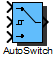
\includegraphics{AutoSwitch}\end{figure} 

\begin{XtoCtabular}{Inports}
In1 & Input \#1\tabularnewline
\hline
Switch & Input \#2: Threshold signal\tabularnewline
\hline
In3 & Input \#3\tabularnewline
\hline
\end{XtoCtabular}


\begin{XtoCtabular}{Outports}
Out & Either value of input \#1 or input \#3 dependent on value of input \#2\tabularnewline
\hline
\end{XtoCtabular}

\begin{XtoCtabular}{Mask Parameters}
Thresh\_up & Threshold level for rising switch signal\tabularnewline
\hline
Thresh\_down & Threshold level for falling switch signal\tabularnewline
\hline
\end{XtoCtabular}

\subsubsection*{Description:}
Switch between In1 and In3 dependent on Switch signal:

    Switch signal rising:  Switch >= Threshold up --> Out = In1

    Switch signal falling: Switch <  Threshold down --> Out = In3

% include optional documentation file
\InputIfFileExists{\XcHomePath/Library/General/Doc/AutoSwitch_Info.tex}{\vspace{1ex}}{}

\subsubsection*{Implementations:}
\begin{tabular}{l l}
\textbf{FiP8} & 8 Bit Fixed Point Implementation\tabularnewline
\textbf{FiP16} & 16 Bit Fixed Point Implementation\tabularnewline
\textbf{FiP32} & 32 Bit Fixed Point Implementation\tabularnewline
\textbf{Float32} & 32 Bit Floating Point Implementation\tabularnewline
\textbf{Float64} & 64 Bit Floating Point Implementation\tabularnewline
\end{tabular}

\XtoCImplementation{FiP8}
\index{Block ID!128}
\nopagebreak[0]
% Implementation details
\begin{tabular}{l l}
\textbf{Name} & FiP8 \tabularnewline
\textbf{ID} & 128 \tabularnewline
\textbf{Revision} & 0.1 \tabularnewline
\textbf{C filename} & AutoSwitch\_FiP8.c \tabularnewline
\textbf{H filename} & AutoSwitch\_FiP8.h \tabularnewline
\end{tabular}
\vspace{1ex}

8 Bit Fixed Point Implementation

\begin{XtoCtabular}{Controller Parameters}
Thresh\_up & Threshold level for rising switch signal\tabularnewline
\hline
Thresh\_down & Threshold level for falling switch signal\tabularnewline
\hline
Status & Current hysteresis state\tabularnewline
\hline
\end{XtoCtabular}

% Implementation data structure
\XtoCDataStruct{Data Structure:}
\begin{lstlisting}
typedef struct {
     uint16        ID;
     int8          *In1;
     int8          *Switch;
     int8          *In3;
     int8          Out;
     int8          Thresh_up;
     int8          Thresh_down;
     int8          Status;
} AUTOSWITCH_FIP8;
\end{lstlisting}

\ifdefined \AddTestReports
\InputIfFileExists{\XcHomePath/Library/General/Doc/Test_AutoSwitch_FiP8.tex}{}{}
\fi
\XtoCImplementation{FiP16}
\index{Block ID!129}
\nopagebreak[0]
% Implementation details
\begin{tabular}{l l}
\textbf{Name} & FiP16 \tabularnewline
\textbf{ID} & 129 \tabularnewline
\textbf{Revision} & 0.1 \tabularnewline
\textbf{C filename} & AutoSwitch\_FiP16.c \tabularnewline
\textbf{H filename} & AutoSwitch\_FiP16.h \tabularnewline
\end{tabular}
\vspace{1ex}

16 Bit Fixed Point Implementation

\begin{XtoCtabular}{Controller Parameters}
Thresh\_up & Threshold level for rising switch signal\tabularnewline
\hline
Thresh\_down & Threshold level for falling switch signal\tabularnewline
\hline
Status & Current hysteresis state\tabularnewline
\hline
\end{XtoCtabular}

% Implementation data structure
\XtoCDataStruct{Data Structure:}
\begin{lstlisting}
typedef struct {
     uint16        ID;
     int16         *In1;
     int16         *Switch;
     int16         *In3;
     int16         Out;
     int16         Thresh_up;
     int16         Thresh_down;
     int8          Status;
} AUTOSWITCH_FIP16;
\end{lstlisting}

\ifdefined \AddTestReports
\InputIfFileExists{\XcHomePath/Library/General/Doc/Test_AutoSwitch_FiP16.tex}{}{}
\fi
\XtoCImplementation{FiP32}
\index{Block ID!130}
\nopagebreak[0]
% Implementation details
\begin{tabular}{l l}
\textbf{Name} & FiP32 \tabularnewline
\textbf{ID} & 130 \tabularnewline
\textbf{Revision} & 0.1 \tabularnewline
\textbf{C filename} & AutoSwitch\_FiP32.c \tabularnewline
\textbf{H filename} & AutoSwitch\_FiP32.h \tabularnewline
\end{tabular}
\vspace{1ex}

32 Bit Fixed Point Implementation

\begin{XtoCtabular}{Controller Parameters}
Thresh\_up & Threshold level for rising switch signal\tabularnewline
\hline
Thresh\_down & Threshold level for falling switch signal\tabularnewline
\hline
Status & Current hysteresis state\tabularnewline
\hline
\end{XtoCtabular}

% Implementation data structure
\XtoCDataStruct{Data Structure:}
\begin{lstlisting}
typedef struct {
     uint16        ID;
     int32         *In1;
     int32         *Switch;
     int32         *In3;
     int32         Out;
     int32         Thresh_up;
     int32         Thresh_down;
     int8          Status;
} AUTOSWITCH_FIP32;
\end{lstlisting}

\ifdefined \AddTestReports
\InputIfFileExists{\XcHomePath/Library/General/Doc/Test_AutoSwitch_FiP32.tex}{}{}
\fi
\XtoCImplementation{Float32}
\index{Block ID!131}
\nopagebreak[0]
% Implementation details
\begin{tabular}{l l}
\textbf{Name} & Float32 \tabularnewline
\textbf{ID} & 131 \tabularnewline
\textbf{Revision} & 0.1 \tabularnewline
\textbf{C filename} & AutoSwitch\_Float32.c \tabularnewline
\textbf{H filename} & AutoSwitch\_Float32.h \tabularnewline
\end{tabular}
\vspace{1ex}

32 Bit Floating Point Implementation

\begin{XtoCtabular}{Controller Parameters}
Thresh\_up & Threshold level for rising switch signal\tabularnewline
\hline
Thresh\_down & Threshold level for falling switch signal\tabularnewline
\hline
Status & Current hysteresis state\tabularnewline
\hline
\end{XtoCtabular}

% Implementation data structure
\XtoCDataStruct{Data Structure:}
\begin{lstlisting}
typedef struct {
     uint16        ID;
     float32       *In1;
     float32       *Switch;
     float32       *In3;
     float32       Out;
     float32       Thresh_up;
     float32       Thresh_down;
     int8          Status;
} AUTOSWITCH_FLOAT32;
\end{lstlisting}

\ifdefined \AddTestReports
\InputIfFileExists{\XcHomePath/Library/General/Doc/Test_AutoSwitch_Float32.tex}{}{}
\fi
\XtoCImplementation{Float64}
\index{Block ID!132}
\nopagebreak[0]
% Implementation details
\begin{tabular}{l l}
\textbf{Name} & Float64 \tabularnewline
\textbf{ID} & 132 \tabularnewline
\textbf{Revision} & 0.1 \tabularnewline
\textbf{C filename} & AutoSwitch\_Float64.c \tabularnewline
\textbf{H filename} & AutoSwitch\_Float64.h \tabularnewline
\end{tabular}
\vspace{1ex}

64 Bit Floating Point Implementation

\begin{XtoCtabular}{Controller Parameters}
Thresh\_up & Threshold level for rising switch signal\tabularnewline
\hline
Thresh\_down & Threshold level for falling switch signal\tabularnewline
\hline
Status & Current hysteresis state\tabularnewline
\hline
\end{XtoCtabular}

% Implementation data structure
\XtoCDataStruct{Data Structure:}
\begin{lstlisting}
typedef struct {
     uint16        ID;
     float64       *In1;
     float64       *Switch;
     float64       *In3;
     float64       Out;
     float64       Thresh_up;
     float64       Thresh_down;
     int8          Status;
} AUTOSWITCH_FLOAT64;
\end{lstlisting}

\ifdefined \AddTestReports
\InputIfFileExists{\XcHomePath/Library/General/Doc/Test_AutoSwitch_Float64.tex}{}{}
\fi
